\documentclass{article}\usepackage[]{graphicx}\usepackage[]{color}
%% maxwidth is the original width if it is less than linewidth
%% otherwise use linewidth (to make sure the graphics do not exceed the margin)
\makeatletter
\def\maxwidth{ %
  \ifdim\Gin@nat@width>\linewidth
    \linewidth
  \else
    \Gin@nat@width
  \fi
}
\makeatother

\definecolor{fgcolor}{rgb}{0.345, 0.345, 0.345}
\newcommand{\hlnum}[1]{\textcolor[rgb]{0.686,0.059,0.569}{#1}}%
\newcommand{\hlstr}[1]{\textcolor[rgb]{0.192,0.494,0.8}{#1}}%
\newcommand{\hlcom}[1]{\textcolor[rgb]{0.678,0.584,0.686}{\textit{#1}}}%
\newcommand{\hlopt}[1]{\textcolor[rgb]{0,0,0}{#1}}%
\newcommand{\hlstd}[1]{\textcolor[rgb]{0.345,0.345,0.345}{#1}}%
\newcommand{\hlkwa}[1]{\textcolor[rgb]{0.161,0.373,0.58}{\textbf{#1}}}%
\newcommand{\hlkwb}[1]{\textcolor[rgb]{0.69,0.353,0.396}{#1}}%
\newcommand{\hlkwc}[1]{\textcolor[rgb]{0.333,0.667,0.333}{#1}}%
\newcommand{\hlkwd}[1]{\textcolor[rgb]{0.737,0.353,0.396}{\textbf{#1}}}%

\usepackage{framed}
\makeatletter
\newenvironment{kframe}{%
 \def\at@end@of@kframe{}%
 \ifinner\ifhmode%
  \def\at@end@of@kframe{\end{minipage}}%
  \begin{minipage}{\columnwidth}%
 \fi\fi%
 \def\FrameCommand##1{\hskip\@totalleftmargin \hskip-\fboxsep
 \colorbox{shadecolor}{##1}\hskip-\fboxsep
     % There is no \\@totalrightmargin, so:
     \hskip-\linewidth \hskip-\@totalleftmargin \hskip\columnwidth}%
 \MakeFramed {\advance\hsize-\width
   \@totalleftmargin\z@ \linewidth\hsize
   \@setminipage}}%
 {\par\unskip\endMakeFramed%
 \at@end@of@kframe}
\makeatother

\definecolor{shadecolor}{rgb}{.97, .97, .97}
\definecolor{messagecolor}{rgb}{0, 0, 0}
\definecolor{warningcolor}{rgb}{1, 0, 1}
\definecolor{errorcolor}{rgb}{1, 0, 0}
\newenvironment{knitrout}{}{} % an empty environment to be redefined in TeX

\usepackage{alltt}

\title{Missing values and modelling in R}
\author{Ken Butler}
\IfFileExists{upquote.sty}{\usepackage{upquote}}{}
\begin{document}

\maketitle

\section{Introduction}

In class today, we were working with the lung cancer data set from the
\texttt{survival} package. This had some missing data in it:

\begin{knitrout}
\definecolor{shadecolor}{rgb}{0.969, 0.969, 0.969}\color{fgcolor}\begin{kframe}
\begin{alltt}
\hlkwd{library}\hlstd{(survival)}
\hlkwd{head}\hlstd{(lung,}\hlnum{10}\hlstd{)}
\end{alltt}
\begin{verbatim}
##    inst time status age sex ph.ecog ph.karno pat.karno meal.cal wt.loss
## 1     3  306      2  74   1       1       90       100     1175      NA
## 2     3  455      2  68   1       0       90        90     1225      15
## 3     3 1010      1  56   1       0       90        90       NA      15
## 4     5  210      2  57   1       1       90        60     1150      11
## 5     1  883      2  60   1       0      100        90       NA       0
## 6    12 1022      1  74   1       1       50        80      513       0
## 7     7  310      2  68   2       2       70        60      384      10
## 8    11  361      2  71   2       2       60        80      538       1
## 9     1  218      2  53   1       1       70        80      825      16
## 10    7  166      2  61   1       2       70        70      271      34
\end{verbatim}
\end{kframe}
\end{knitrout}

You might have been wondering why (a) I could fit models, but (b) why
I could \emph{not} do \texttt{anova} and suchlike things (which I
really ought to have done, from a data analysis point of view.)

\section{Complete cases}

An observation (row) of the data frame that has values for all the variables
is called a \textbf{complete case}. Or, if there are any missing
values anywhere along the row, it is \emph{not} a complete case.

In the lung cancer data frame excerpt above, rows 1, 3 and 5 have
missing values in them somewhere, but the other rows are all complete cases.

R has a function called \texttt{complete.cases} that takes a data
frame and returns \texttt{TRUE} if that row is a complete case and
\texttt{FALSE} if it has any missing values anywhere. Here is the
output from running \texttt{complete.cases} on the first 10 rows of
our data frame:

\begin{knitrout}
\definecolor{shadecolor}{rgb}{0.969, 0.969, 0.969}\color{fgcolor}\begin{kframe}
\begin{alltt}
\hlstd{v}\hlkwb{=}\hlkwd{complete.cases}\hlstd{(lung)}
\hlstd{v[}\hlnum{1}\hlopt{:}\hlnum{10}\hlstd{]}
\end{alltt}
\begin{verbatim}
##  [1] FALSE  TRUE FALSE  TRUE FALSE  TRUE  TRUE  TRUE  TRUE  TRUE
\end{verbatim}
\end{kframe}
\end{knitrout}

Or, more precisely, of running it on the whole data frame and showing
you the first ten values. Values 1, 3 and 5 are \texttt{FALSE},
corresponding to those rows having missing values in them somewhere,
and the other values are \texttt{TRUE}, meaning that those rows are
complete cases with no missing values.

When we fit a model, only the relevantly complete cases are used (I
expand on this in a moment). The simplest situation is if the model has all
the explanatory variables in it, like this:

\begin{knitrout}
\definecolor{shadecolor}{rgb}{0.969, 0.969, 0.969}\color{fgcolor}\begin{kframe}
\begin{alltt}
\hlkwd{attach}\hlstd{(lung)}
\hlstd{resp}\hlkwb{=}\hlkwd{Surv}\hlstd{(time,status}\hlopt{==}\hlnum{2}\hlstd{)}
\hlstd{lung.1}\hlkwb{=}\hlkwd{coxph}\hlstd{(resp}\hlopt{~}\hlstd{age}\hlopt{+}\hlstd{sex}\hlopt{+}\hlstd{ph.ecog}\hlopt{+}\hlstd{ph.karno}\hlopt{+}\hlstd{pat.karno}\hlopt{+}
  \hlstd{meal.cal}\hlopt{+}\hlstd{wt.loss)}
\hlkwd{summary}\hlstd{(lung.1)}
\end{alltt}
\begin{verbatim}
## Call:
## coxph(formula = resp ~ age + sex + ph.ecog + ph.karno + pat.karno + 
##     meal.cal + wt.loss)
## 
##   n= 168, number of events= 121 
##    (60 observations deleted due to missingness)
## 
##                 coef  exp(coef)   se(coef)      z Pr(>|z|)   
## age        1.065e-02  1.011e+00  1.161e-02  0.917  0.35906   
## sex       -5.509e-01  5.765e-01  2.008e-01 -2.743  0.00609 **
## ph.ecog    7.342e-01  2.084e+00  2.233e-01  3.288  0.00101 **
## ph.karno   2.246e-02  1.023e+00  1.124e-02  1.998  0.04574 * 
## pat.karno -1.242e-02  9.877e-01  8.054e-03 -1.542  0.12316   
## meal.cal   3.329e-05  1.000e+00  2.595e-04  0.128  0.89791   
## wt.loss   -1.433e-02  9.858e-01  7.771e-03 -1.844  0.06518 . 
## ---
## Signif. codes:  0 '***' 0.001 '**' 0.01 '*' 0.05 '.' 0.1 ' ' 1
## 
##           exp(coef) exp(-coef) lower .95 upper .95
## age          1.0107     0.9894    0.9880    1.0340
## sex          0.5765     1.7347    0.3889    0.8545
## ph.ecog      2.0838     0.4799    1.3452    3.2277
## ph.karno     1.0227     0.9778    1.0004    1.0455
## pat.karno    0.9877     1.0125    0.9722    1.0034
## meal.cal     1.0000     1.0000    0.9995    1.0005
## wt.loss      0.9858     1.0144    0.9709    1.0009
## 
## Concordance= 0.651  (se = 0.031 )
## Rsquare= 0.155   (max possible= 0.998 )
## Likelihood ratio test= 28.33  on 7 df,   p=0.0001918
## Wald test            = 27.58  on 7 df,   p=0.0002616
## Score (logrank) test = 28.41  on 7 df,   p=0.0001849
\end{verbatim}
\end{kframe}
\end{knitrout}

This uses 168 observations (as the output shows). This is how many
complete cases there are:

\begin{knitrout}
\definecolor{shadecolor}{rgb}{0.969, 0.969, 0.969}\color{fgcolor}\begin{kframe}
\begin{alltt}
\hlkwd{table}\hlstd{(v)}
\end{alltt}
\begin{verbatim}
## v
## FALSE  TRUE 
##    61   167
\end{verbatim}
\end{kframe}
\end{knitrout}

Oh, not quite the same. But I can explain that too. I explain that in a minute,
but this is relevant in the meanwhile:

\begin{knitrout}
\definecolor{shadecolor}{rgb}{0.969, 0.969, 0.969}\color{fgcolor}\begin{kframe}
\begin{alltt}
\hlkwd{summary}\hlstd{(lung)}
\end{alltt}
\begin{verbatim}
##       inst            time            status           age       
##  Min.   : 1.00   Min.   :   5.0   Min.   :1.000   Min.   :39.00  
##  1st Qu.: 3.00   1st Qu.: 166.8   1st Qu.:1.000   1st Qu.:56.00  
##  Median :11.00   Median : 255.5   Median :2.000   Median :63.00  
##  Mean   :11.09   Mean   : 305.2   Mean   :1.724   Mean   :62.45  
##  3rd Qu.:16.00   3rd Qu.: 396.5   3rd Qu.:2.000   3rd Qu.:69.00  
##  Max.   :33.00   Max.   :1022.0   Max.   :2.000   Max.   :82.00  
##  NA's   :1                                                       
##       sex           ph.ecog          ph.karno        pat.karno     
##  Min.   :1.000   Min.   :0.0000   Min.   : 50.00   Min.   : 30.00  
##  1st Qu.:1.000   1st Qu.:0.0000   1st Qu.: 75.00   1st Qu.: 70.00  
##  Median :1.000   Median :1.0000   Median : 80.00   Median : 80.00  
##  Mean   :1.395   Mean   :0.9515   Mean   : 81.94   Mean   : 79.96  
##  3rd Qu.:2.000   3rd Qu.:1.0000   3rd Qu.: 90.00   3rd Qu.: 90.00  
##  Max.   :2.000   Max.   :3.0000   Max.   :100.00   Max.   :100.00  
##                  NA's   :1        NA's   :1        NA's   :3       
##     meal.cal         wt.loss       
##  Min.   :  96.0   Min.   :-24.000  
##  1st Qu.: 635.0   1st Qu.:  0.000  
##  Median : 975.0   Median :  7.000  
##  Mean   : 928.8   Mean   :  9.832  
##  3rd Qu.:1150.0   3rd Qu.: 15.750  
##  Max.   :2600.0   Max.   : 68.000  
##  NA's   :47       NA's   :14
\end{verbatim}
\end{kframe}
\end{knitrout}

Now, suppose I decide to take out \texttt{meal.cal} since that is
nowhere near significant. I could go blindly like this, and wonder
what happened:

\begin{knitrout}
\definecolor{shadecolor}{rgb}{0.969, 0.969, 0.969}\color{fgcolor}\begin{kframe}
\begin{alltt}
\hlstd{lung.2}\hlkwb{=}\hlkwd{coxph}\hlstd{(resp}\hlopt{~}\hlstd{age}\hlopt{+}\hlstd{sex}\hlopt{+}\hlstd{ph.ecog}\hlopt{+}\hlstd{ph.karno}\hlopt{+}\hlstd{pat.karno}\hlopt{+}\hlstd{wt.loss)}
\hlkwd{anova}\hlstd{(lung.2,lung.1)}
\end{alltt}


{\ttfamily\noindent\bfseries\color{errorcolor}{\#\# Error in anova.coxphlist(c(list(object), dotargs), test = test): models were not all fitted to the same size of dataset}}\end{kframe}
\end{knitrout}

The answer to this riddle is found by looking at the \texttt{summary}
of our smaller model:

\begin{knitrout}
\definecolor{shadecolor}{rgb}{0.969, 0.969, 0.969}\color{fgcolor}\begin{kframe}
\begin{alltt}
\hlkwd{summary}\hlstd{(lung.2)}
\end{alltt}
\begin{verbatim}
## Call:
## coxph(formula = resp ~ age + sex + ph.ecog + ph.karno + pat.karno + 
##     wt.loss)
## 
##   n= 210, number of events= 148 
##    (18 observations deleted due to missingness)
## 
##                coef exp(coef)  se(coef)      z Pr(>|z|)    
## age        0.013058  1.013144  0.009866  1.324 0.185639    
## sex       -0.625167  0.535172  0.178703 -3.498 0.000468 ***
## ph.ecog    0.675227  1.964479  0.198735  3.398 0.000680 ***
## ph.karno   0.020116  1.020320  0.010178  1.976 0.048111 *  
## pat.karno -0.014743  0.985365  0.007300 -2.019 0.043440 *  
## wt.loss   -0.013243  0.986844  0.007009 -1.889 0.058836 .  
## ---
## Signif. codes:  0 '***' 0.001 '**' 0.01 '*' 0.05 '.' 0.1 ' ' 1
## 
##           exp(coef) exp(-coef) lower .95 upper .95
## age          1.0131     0.9870    0.9937    1.0329
## sex          0.5352     1.8686    0.3770    0.7596
## ph.ecog      1.9645     0.5090    1.3307    2.9001
## ph.karno     1.0203     0.9801    1.0002    1.0409
## pat.karno    0.9854     1.0149    0.9714    0.9996
## wt.loss      0.9868     1.0133    0.9734    1.0005
## 
## Concordance= 0.656  (se = 0.028 )
## Rsquare= 0.162   (max possible= 0.998 )
## Likelihood ratio test= 37.2  on 6 df,   p=1.611e-06
## Wald test            = 36.49  on 6 df,   p=2.209e-06
## Score (logrank) test = 37.59  on 6 df,   p=1.352e-06
\end{verbatim}
\end{kframe}
\end{knitrout}

The model \texttt{lung.2} without \texttt{meal.cal} is based on 210 observations, much
more than the 168 observations on which \texttt{lung.1} was based. We
can't very well compare two models fit to different data, and indeed
\texttt{anova} won't let us do that (that was the error message).

Why the big difference? Let's look at the top of the data frame again:

\begin{knitrout}
\definecolor{shadecolor}{rgb}{0.969, 0.969, 0.969}\color{fgcolor}\begin{kframe}
\begin{alltt}
\hlkwd{head}\hlstd{(lung)}
\end{alltt}
\begin{verbatim}
##   inst time status age sex ph.ecog ph.karno pat.karno meal.cal wt.loss
## 1    3  306      2  74   1       1       90       100     1175      NA
## 2    3  455      2  68   1       0       90        90     1225      15
## 3    3 1010      1  56   1       0       90        90       NA      15
## 4    5  210      2  57   1       1       90        60     1150      11
## 5    1  883      2  60   1       0      100        90       NA       0
## 6   12 1022      1  74   1       1       50        80      513       0
\end{verbatim}
\end{kframe}
\end{knitrout}

Take a look at rows 3 and 5. These observations are missing
\texttt{meal.cal} but nothing else. So, as far as a model without
\texttt{meal.cal} is concerned, these are now complete cases, because
they have values for all the variables that feature in the model. That
is what I meant by ``relevantly complete'': rows 3 and 5 (and
evidently a lot of others) are complete cases as far as
\texttt{lung.2} is concerned, which is why \texttt{lung.2} is based on
a lot more observations than \texttt{lung.1}. If you look at the
output to \texttt{summary(lung)} above (the summary of the data
frame), you'll see that \texttt{meal.cal} has 47 missing
observations. Some of these (though probably not many) are going to
have other missing values as well (and therefore aren't in
\texttt{lung.2} either), but most of them will have the
\texttt{meal.cal} as the only missing value, and therefore they will
be included in \texttt{lung.2} but not in \texttt{lung.1}.

So why did I have 168 observations in \texttt{lung.1} but only 167
complete cases? ``Relevantly complete'' is the answer here too. One
observation has a missing value for \texttt{inst} but is otherwise
complete. Since \texttt{inst} didn't feature in \texttt{lung.1}, this
observation is a complete case for \texttt{lung.1}.

This all explains my rather cavalier treatment of model-building in
class. The only other way I could go is to deliberately remove the one
least significant explanatory variable at a time, and that would have
taken too long in class.

\section{Using only the complete cases}

The other option is to throw out all the observations with any missing
values before you start. That way, you know that all your analyses are
based on the same data set, and the issue of ``relevantly complete''
is, um, irrelevant. If you do that, you might lose a lot of data off
the top, but you have all the apparatus of model-building available to you.

How to keep only the complete cases? Remember the function \texttt{complete.cases}?
That was \texttt{TRUE} if the row was complete and \texttt{FALSE} if
it had any missing values. We can use that to select only the rows
without missings like this:

\begin{knitrout}
\definecolor{shadecolor}{rgb}{0.969, 0.969, 0.969}\color{fgcolor}\begin{kframe}
\begin{alltt}
\hlstd{v}\hlkwb{=}\hlkwd{complete.cases}\hlstd{(lung)}
\hlstd{lung.nom}\hlkwb{=}\hlstd{lung[v,]}
\hlkwd{head}\hlstd{(lung.nom)}
\end{alltt}
\begin{verbatim}
##   inst time status age sex ph.ecog ph.karno pat.karno meal.cal wt.loss
## 2    3  455      2  68   1       0       90        90     1225      15
## 4    5  210      2  57   1       1       90        60     1150      11
## 6   12 1022      1  74   1       1       50        80      513       0
## 7    7  310      2  68   2       2       70        60      384      10
## 8   11  361      2  71   2       2       60        80      538       1
## 9    1  218      2  53   1       1       70        80      825      16
\end{verbatim}
\end{kframe}
\end{knitrout}

No missing values here (or, presumably, anywhere else in
\texttt{lung.nom}). Note that the row numbers come from the
\emph{original} data frame, rows 1, 3 and 5 of which must have had
(and did have) missing values. \texttt{lung.nom} ought to have 167
rows, since that's how many completely complete cases we had:

\begin{knitrout}
\definecolor{shadecolor}{rgb}{0.969, 0.969, 0.969}\color{fgcolor}\begin{kframe}
\begin{alltt}
\hlkwd{dim}\hlstd{(lung.nom)}
\end{alltt}
\begin{verbatim}
## [1] 167  10
\end{verbatim}
\end{kframe}
\end{knitrout}

If you like \texttt{dplyr}, you can also pull out the complete cases
that way. The smartest thing is to save the result of
\texttt{complete.cases} \emph{inside} the data frame:

\begin{knitrout}
\definecolor{shadecolor}{rgb}{0.969, 0.969, 0.969}\color{fgcolor}\begin{kframe}
\begin{alltt}
\hlkwd{library}\hlstd{(dplyr)}
\end{alltt}


{\ttfamily\noindent\itshape\color{messagecolor}{\#\# \\\#\# Attaching package: 'dplyr'}}

{\ttfamily\noindent\itshape\color{messagecolor}{\#\# The following objects are masked from 'package:stats':\\\#\# \\\#\#\ \ \ \  filter, lag}}

{\ttfamily\noindent\itshape\color{messagecolor}{\#\# The following objects are masked from 'package:base':\\\#\# \\\#\#\ \ \ \  intersect, setdiff, setequal, union}}\begin{alltt}
\hlstd{lung} \hlopt \hlkwd{mutate}\hlstd{(}\hlkwc{comp}\hlstd{=}\hlkwd{complete.cases}\hlstd{(lung))} \hlopt \hlkwd{filter}\hlstd{(comp)} \hlkwb{->} \hlstd{lung.nom}
\hlkwd{dim}\hlstd{(lung.nom)}
\end{alltt}
\begin{verbatim}
## [1] 167  11
\end{verbatim}
\end{kframe}
\end{knitrout}

The extra column is that \texttt{comp} I created, which will be
completely \texttt{TRUE} in \texttt{lung.nom}.

\section{Modelling with the complete cases}

If we use the data frame \texttt{lung.nom} with no missing values, we
have all the modelling machinery available to us. But we have to go
back and start again:

\begin{knitrout}
\definecolor{shadecolor}{rgb}{0.969, 0.969, 0.969}\color{fgcolor}\begin{kframe}
\begin{alltt}
\hlkwd{detach}\hlstd{(lung)}
\hlkwd{attach}\hlstd{(lung.nom)}
\hlstd{y}\hlkwb{=}\hlkwd{Surv}\hlstd{(time,status}\hlopt{==}\hlnum{2}\hlstd{)}
\hlstd{lung.nom.1}\hlkwb{=}\hlkwd{coxph}\hlstd{(y}\hlopt{~}\hlstd{age}\hlopt{+}\hlstd{sex}\hlopt{+}\hlstd{ph.ecog}\hlopt{+}\hlstd{ph.karno}\hlopt{+}\hlstd{pat.karno}\hlopt{+}\hlstd{meal.cal}\hlopt{+}\hlstd{wt.loss)}
\hlstd{lung.nom.2}\hlkwb{=}\hlkwd{update}\hlstd{(lung.nom.1,.}\hlopt{~}\hlstd{.}\hlopt{-}\hlstd{meal.cal)}
\hlkwd{anova}\hlstd{(lung.nom.2,lung.nom.1)}
\end{alltt}
\begin{verbatim}
## Analysis of Deviance Table
##  Cox model: response is  y
##  Model 1: ~ age + sex + ph.ecog + ph.karno + pat.karno + wt.loss
##  Model 2: ~ age + sex + ph.ecog + ph.karno + pat.karno + meal.cal + wt.loss
##    loglik  Chisq Df P(>|Chi|)
## 1 -494.04                    
## 2 -494.03 0.0119  1    0.9132
\end{verbatim}
\end{kframe}
\end{knitrout}

We can also use \texttt{drop1} to help us decide what should come out next:

\begin{knitrout}
\definecolor{shadecolor}{rgb}{0.969, 0.969, 0.969}\color{fgcolor}\begin{kframe}
\begin{alltt}
\hlkwd{drop1}\hlstd{(lung.nom.2,}\hlkwc{test}\hlstd{=}\hlstr{"Chisq"}\hlstd{)}
\end{alltt}
\begin{verbatim}
## Single term deletions
## 
## Model:
## y ~ age + sex + ph.ecog + ph.karno + pat.karno + wt.loss
##           Df     AIC     LRT  Pr(>Chi)    
## <none>       1000.08                      
## age        1  998.95  0.8714 0.3505744    
## sex        1 1006.29  8.2053 0.0041769 ** 
## ph.ecog    1 1009.09 11.0138 0.0009043 ***
## ph.karno   1 1002.28  4.2018 0.0403808 *  
## pat.karno  1 1000.29  2.2073 0.1373553    
## wt.loss    1 1001.60  3.5196 0.0606477 .  
## ---
## Signif. codes:  0 '***' 0.001 '**' 0.01 '*' 0.05 '.' 0.1 ' ' 1
\end{verbatim}
\end{kframe}
\end{knitrout}

It appears to be \texttt{age}.

And if you are lazy (or efficient, depending on your point of view),
you can do the whole elimination in one go:

\begin{knitrout}
\definecolor{shadecolor}{rgb}{0.969, 0.969, 0.969}\color{fgcolor}\begin{kframe}
\begin{alltt}
\hlkwd{step}\hlstd{(lung.nom.1)}
\end{alltt}
\begin{verbatim}
## Start:  AIC=1002.07
## y ~ age + sex + ph.ecog + ph.karno + pat.karno + meal.cal + wt.loss
## 
##             Df    AIC
## - meal.cal   1 1000.1
## - age        1 1001.0
## <none>         1002.1
## - pat.karno  1 1002.3
## - wt.loss    1 1003.6
## - ph.karno   1 1004.3
## - sex        1 1008.0
## - ph.ecog    1 1011.1
## 
## Step:  AIC=1000.08
## y ~ age + sex + ph.ecog + ph.karno + pat.karno + wt.loss
## 
##             Df     AIC
## - age        1  998.95
## <none>         1000.08
## - pat.karno  1 1000.29
## - wt.loss    1 1001.60
## - ph.karno   1 1002.28
## - sex        1 1006.29
## - ph.ecog    1 1009.09
## 
## Step:  AIC=998.95
## y ~ sex + ph.ecog + ph.karno + pat.karno + wt.loss
## 
##             Df     AIC
## <none>          998.95
## - pat.karno  1  999.34
## - ph.karno   1 1000.53
## - wt.loss    1 1000.74
## - sex        1 1005.25
## - ph.ecog    1 1007.83
## Call:
## coxph(formula = y ~ sex + ph.ecog + ph.karno + pat.karno + wt.loss)
## 
## 
##               coef exp(coef) se(coef)     z      p
## sex       -0.55819   0.57224  0.19920 -2.80 0.0051
## ph.ecog    0.74298   2.10220  0.22760  3.26 0.0011
## ph.karno   0.02037   1.02057  0.01108  1.84 0.0660
## pat.karno -0.01240   0.98768  0.00798 -1.55 0.1201
## wt.loss   -0.01449   0.98561  0.00769 -1.88 0.0596
## 
## Likelihood ratio test=27.3  on 5 df, p=5.03e-05
## n= 167, number of events= 120
\end{verbatim}
\end{kframe}
\end{knitrout}

Following the process through, we eliminate \texttt{meal.cal} and then
age, but stop there,
leaving everything else in the model.

This is based on AIC rather than tests, so it can leave some
tangentially relevant variables in the model. 

I think we should now go back and fit this model to the whole data
set, so that we can take advantage of the relevantly-complete cases:

\begin{knitrout}
\definecolor{shadecolor}{rgb}{0.969, 0.969, 0.969}\color{fgcolor}\begin{kframe}
\begin{alltt}
\hlkwd{detach}\hlstd{(lung.nom)}
\hlstd{lung.4}\hlkwb{=}\hlkwd{coxph}\hlstd{(resp}\hlopt{~}\hlstd{sex}\hlopt{+}\hlstd{ph.ecog}\hlopt{+}\hlstd{ph.karno}\hlopt{+}\hlstd{pat.karno}\hlopt{+}\hlstd{wt.loss,}\hlkwc{data}\hlstd{=lung)}
\hlkwd{summary}\hlstd{(lung.4)}
\end{alltt}
\begin{verbatim}
## Call:
## coxph(formula = resp ~ sex + ph.ecog + ph.karno + pat.karno + 
##     wt.loss, data = lung)
## 
##   n= 210, number of events= 148 
##    (18 observations deleted due to missingness)
## 
##                coef exp(coef)  se(coef)      z Pr(>|z|)    
## sex       -0.614915  0.540687  0.177886 -3.457 0.000547 ***
## ph.ecog    0.682441  1.978702  0.201278  3.391 0.000698 ***
## ph.karno   0.018887  1.019066  0.010267  1.840 0.065838 .  
## pat.karno -0.015255  0.984861  0.007306 -2.088 0.036797 *  
## wt.loss   -0.012914  0.987169  0.006844 -1.887 0.059162 .  
## ---
## Signif. codes:  0 '***' 0.001 '**' 0.01 '*' 0.05 '.' 0.1 ' ' 1
## 
##           exp(coef) exp(-coef) lower .95 upper .95
## sex          0.5407     1.8495    0.3815    0.7662
## ph.ecog      1.9787     0.5054    1.3337    2.9357
## ph.karno     1.0191     0.9813    0.9988    1.0398
## pat.karno    0.9849     1.0154    0.9709    0.9991
## wt.loss      0.9872     1.0130    0.9740    1.0005
## 
## Concordance= 0.659  (se = 0.028 )
## Rsquare= 0.155   (max possible= 0.998 )
## Likelihood ratio test= 35.41  on 5 df,   p=1.245e-06
## Wald test            = 35.47  on 5 df,   p=1.214e-06
## Score (logrank) test = 36.33  on 5 df,   p=8.158e-07
\end{verbatim}
\end{kframe}
\end{knitrout}

We had to be careful to use the response variable \texttt{resp} that
came from the \emph{original} data set, not the new one \texttt{y}
that we created from only the complete cases.

The result from \texttt{step} and the model \texttt{lung.4} won't be
exactly the same, because they are based on different data, but the
overall picture should be similar. In each case here, the two
Karnofsky scores and weight loss were teetering on the brink of
significance. 

Also, predictions from
\texttt{lung.4} ought to be better because they are based on more data.

Talking of predictions, how can we do predictions with so many
variables? I think we have to distinguish them by colours:

\begin{knitrout}
\definecolor{shadecolor}{rgb}{0.969, 0.969, 0.969}\color{fgcolor}\begin{kframe}
\begin{alltt}
\hlstd{sexes}\hlkwb{=}\hlkwd{c}\hlstd{(}\hlnum{1}\hlstd{,}\hlnum{2}\hlstd{)}
\hlstd{ph.ecogs}\hlkwb{=}\hlkwd{c}\hlstd{(}\hlnum{0}\hlstd{,}\hlnum{1}\hlstd{)}
\hlstd{ph.karnos}\hlkwb{=}\hlkwd{c}\hlstd{(}\hlnum{75}\hlstd{,}\hlnum{82}\hlstd{)}
\hlstd{pat.karnos}\hlkwb{=}\hlkwd{c}\hlstd{(}\hlnum{70}\hlstd{,}\hlnum{80}\hlstd{)}
\hlstd{wt.losses}\hlkwb{=}\hlkwd{c}\hlstd{(}\hlnum{0}\hlstd{,}\hlnum{16}\hlstd{)}
\end{alltt}
\end{kframe}
\end{knitrout}

We have so many variables, so I only picked two values (the quartiles) for each, to
stop the ``newdata'' data frame from getting too big. As it is, it'll
have $2^5=32$ rows, which is going to make for a very busy plot.

\begin{knitrout}
\definecolor{shadecolor}{rgb}{0.969, 0.969, 0.969}\color{fgcolor}\begin{kframe}
\begin{alltt}
\hlstd{new}\hlkwb{=}\hlkwd{expand.grid}\hlstd{(}\hlkwc{sex}\hlstd{=sexes,}\hlkwc{ph.ecog}\hlstd{=ph.ecogs,}\hlkwc{ph.karno}\hlstd{=ph.karnos,}
  \hlkwc{pat.karno}\hlstd{=pat.karnos,}\hlkwc{wt.loss}\hlstd{=wt.losses)}
\hlstd{pp}\hlkwb{=}\hlkwd{survfit}\hlstd{(lung.4,new)}
\hlkwd{plot}\hlstd{(pp,}\hlkwc{col}\hlstd{=}\hlnum{1}\hlopt{:}\hlnum{32}\hlstd{)}
\end{alltt}
\end{kframe}
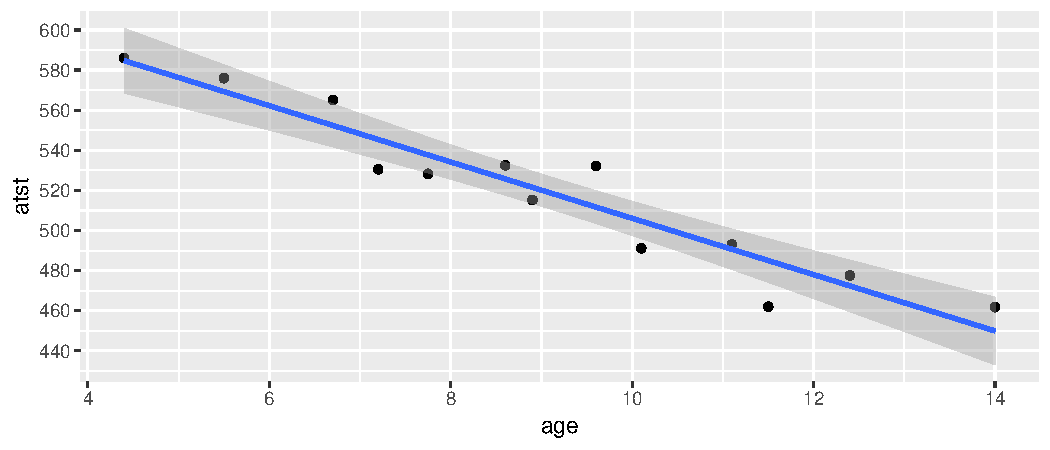
\includegraphics[width=\maxwidth]{figure/unnamed-chunk-17-1} 

\end{knitrout}

Pretty, but very uninformative (there are too many colours to tell
apart). I can't even imagine getting a 32-item legend on there.

Or we go back to the summary of \texttt{lung.4}:

\begin{knitrout}
\definecolor{shadecolor}{rgb}{0.969, 0.969, 0.969}\color{fgcolor}\begin{kframe}
\begin{alltt}
\hlkwd{summary}\hlstd{(lung.4)}\hlopt{$}\hlstd{coefficients}
\end{alltt}
\begin{verbatim}
##                  coef exp(coef)    se(coef)         z     Pr(>|z|)
## sex       -0.61491517 0.5406868 0.177885551 -3.456802 0.0005466258
## ph.ecog    0.68244129 1.9787024 0.201278422  3.390534 0.0006975666
## ph.karno   0.01888670 1.0190662 0.010267173  1.839522 0.0658383733
## pat.karno -0.01525472 0.9848610 0.007305883 -2.088005 0.0367973944
## wt.loss   -0.01291366 0.9871694 0.006843528 -1.886988 0.0591619075
\end{verbatim}
\end{kframe}
\end{knitrout}

What is associated with survival (not dying) is a higher value of
\texttt{sex} (being female), a lower value of \texttt{ph.ecog} (which
makes sense), a lower value of \texttt{ph.karno} (which makes no sense
since higher is supposed to be better), a higher value of
\texttt{pat.karno}, as expected, and oddly a \emph{higher} value of
\texttt{wt.loss}. 

Am I brave enough to try to do this in \texttt{ggplot}? I'm going to
use my function \texttt{ggsurvplot}\footnote{One of the first things
  you learn as a programmer is to re-use what you did before rather
  than reinventing the wheel.} from my solutions to assignment 4
(question 5; see there for what this function does):

\begin{knitrout}
\definecolor{shadecolor}{rgb}{0.969, 0.969, 0.969}\color{fgcolor}\begin{kframe}
\begin{alltt}
\hlstd{ggsurvplot}\hlkwb{=}\hlkwa{function}\hlstd{(}\hlkwc{s}\hlstd{,}\hlkwc{new}\hlstd{) \{}
  \hlcom{# s is output from survfit }
  \hlcom{# new is combos of values that were predicted for}
  \hlstd{newnames}\hlkwb{=}\hlkwd{do.call}\hlstd{(paste,} \hlkwd{c}\hlstd{(new,} \hlkwc{sep}\hlstd{=}\hlstr{"."}\hlstd{))}
  \hlstd{v}\hlkwb{=}\hlkwd{data.frame}\hlstd{(}\hlkwc{time}\hlstd{=s}\hlopt{$}\hlstd{time,}\hlkwc{surv}\hlstd{=s}\hlopt{$}\hlstd{surv)}
  \hlkwd{names}\hlstd{(v)}\hlkwb{=}\hlkwd{c}\hlstd{(}\hlstr{"time"}\hlstd{,newnames)}
  \hlstd{p}\hlkwb{=}\hlkwd{gather}\hlstd{(v,combo,surv,}\hlopt{-}\hlstd{time)}
  \hlkwd{ggplot}\hlstd{(p,}\hlkwd{aes}\hlstd{(}\hlkwc{x}\hlstd{=time,}\hlkwc{y}\hlstd{=surv,}\hlkwc{colour}\hlstd{=combo))}\hlopt{+}
    \hlkwd{geom_point}\hlstd{()}\hlopt{+}\hlkwd{geom_line}\hlstd{()}
\hlstd{\}}
\end{alltt}
\end{kframe}
\end{knitrout}

and then run it:

\begin{knitrout}
\definecolor{shadecolor}{rgb}{0.969, 0.969, 0.969}\color{fgcolor}\begin{kframe}
\begin{alltt}
\hlkwd{library}\hlstd{(tidyr)}
\hlkwd{library}\hlstd{(ggplot2)}
\hlkwd{ggsurvplot}\hlstd{(pp,new)}
\end{alltt}
\end{kframe}
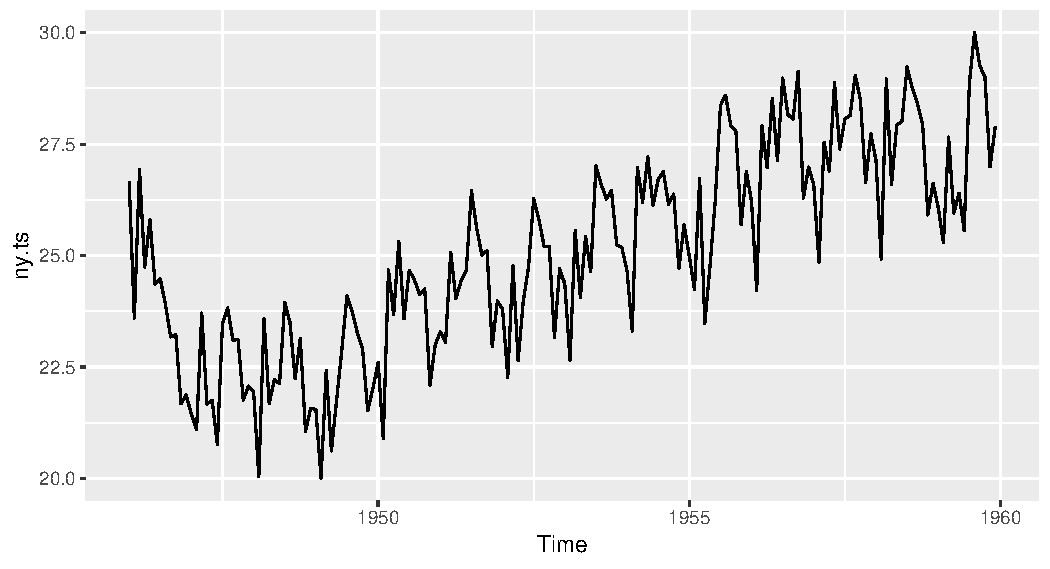
\includegraphics[width=\maxwidth]{figure/unnamed-chunk-20-1} 

\end{knitrout}

Good luck picking out the colour of the best combination! The labels
on the legend are the values of the five variables in the order that we put them in
\texttt{new} (that is, the same order as in the
\texttt{expand.grid}). I think the best one ought to be
\texttt{2.0.75.80.16} (those are respectively high, low, low, high,
high of the values we chose for those five variables). Which is
certainly one of those blue ones, but I'm not sure whether it's
\emph{that} one.

Qualitatively, the best survival curves are the blue and purple ones
(females with the best ECOG score of zero), and the worst ones are the
green ones (males with the worse ECOG score of 1). The better-ECOG
males (orange) and the worse-ECOG females (pink) are all  mixed up in
the middle.

\end{document}

